% geometry_and_trigonometry:x05 GDC:YES
\begin{question}
  \hspace*{\fill} [Note Maximale: 6]\par
  \medskip
  \noindent La figure suivante montre $\bigtriangleup\,PQR$, tel que $RQ = 9\,cm$, $\angle\,PRQ = 70^\circ$. $\angle\,PQR = 45^\circ$.\par
  \medskip
  \begin{center} % or flushleft or flushright
    \noindent La figure n'est pas à l'échelle.\par
    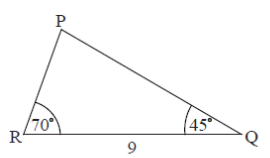
\includegraphics[scale=0.4]{figure_x5}\par
  \end{center} % or flushleft or flushright
  \begin{enumerate}[label=(\alph*)]
    \item Trouvez $\angle\,RPQ$.\hspace*{\fill} [1]
    \item Trouvez $PR$.\hspace*{\fill} [3]
    \item Trouvez l'aire de $\bigtriangleup\,PQR$.\hspace*{\fill} [2]
  \end{enumerate}
\end{question}
